\documentclass[.../Dokumentation.tex]{subfiles}
\begin{document}
\subsection{Darstellung}\label{sec-ita3-visualization}
Da wegen der Dimensionen der Servomotoren keine zufriedenstellende Lösung 
mit in den Ästen integrierten Motoren gefunden werden konnte, wurde ein neues 
Konzept erarbeitet.
Während an der Idee, den Baum in einer mit LEDs umrandeten Kiste zu montieren, 
festgehalten wurde, sah der neue Ansatz vor, die Äste des Baums über Schnüre 
oder Ähnliches zu bewegen.
Diese sollen idealerweise von oberhalb des Baums, bewegt durch die Servomotoren, 
eine marionettenartige Funktionalität herstellen.
Der schematische Aufbau dieser Lösung ist in Abbildung \ref{fig-treeNew} 
dargestellt.
\begin{figure}[H]
\begin{center}
    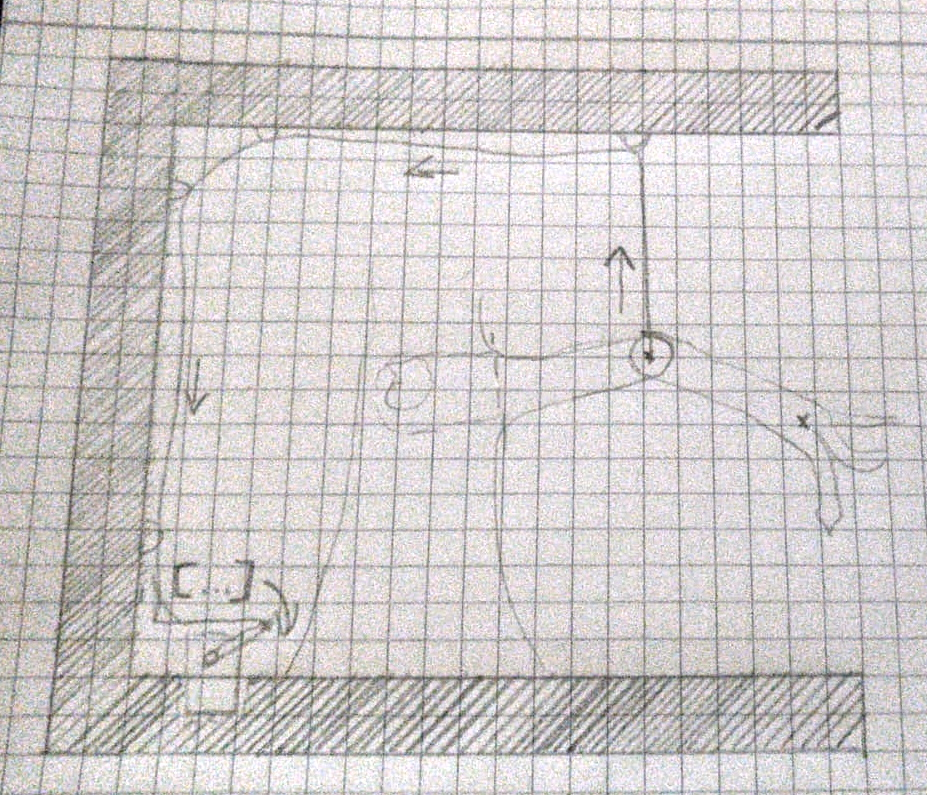
\includegraphics[
        width=0.5\linewidth,
    ]{imgs/treeNew.jpg}
    \caption{Überarbeitetes Darstellungskonzept}
    \label{fig-treeNew}
\end{center}
\end{figure}
\noindent
Aufgrund der Tatsache, dass sich keine geeignete Umsetzung des Baums  
mittels 3D-Druck erzielen ließ, wurde ein Bild einer Baumsilhouette gesucht.
Mit diesem war es unter der Vorraussetzung eines geeigneten Formats möglich, 
einen qualitativ 
hochwertigen Baum mit Hilfe des Lasercutters des \textit{FabLab}s herzustellen.
Auf dem gleichen Weg war es weiter ein Leichtes, die benötigte Kiste zu 
realisieren \footnote{https://de.makercase.com/\#/basicbox}.
In Abbildung \ref{fig-tree-in-box} ist ein erster Eindruck hiervon zu sehen.
\begin{figure}[H]
\begin{center}
    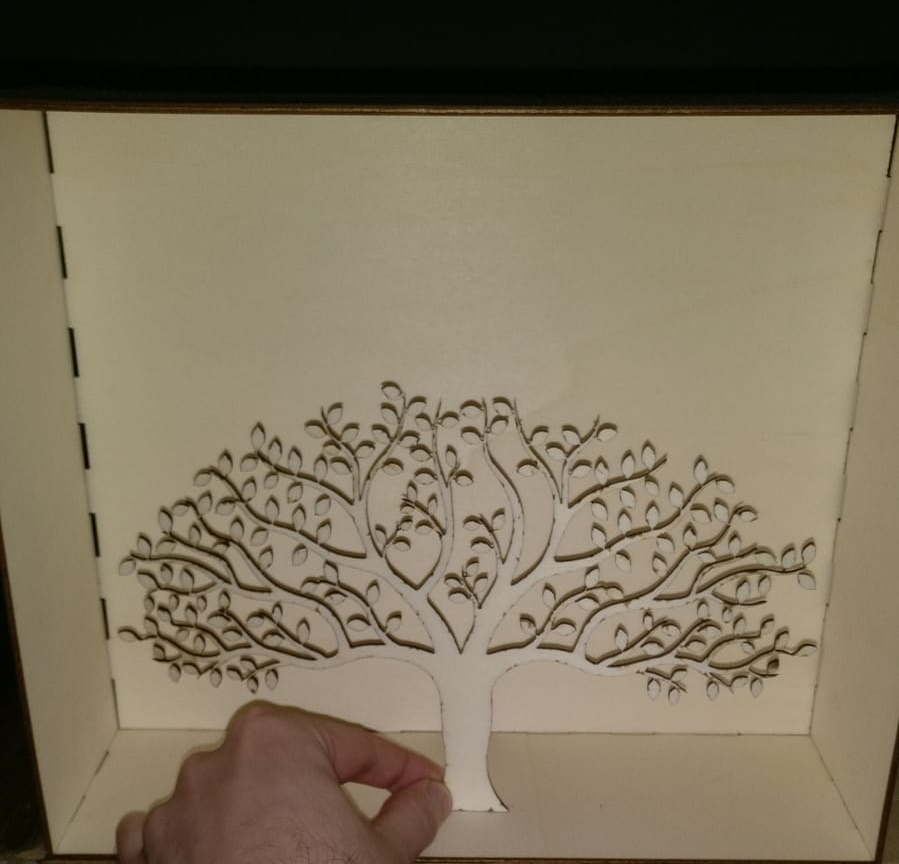
\includegraphics[
        width=0.5\linewidth,
    ]{imgs/tree_in_box.jpeg}
    \caption{Ausgeschnittener Baum in Kiste}
    \label{fig-tree-in-box}
\end{center}
\end{figure}
\end{document}